\documentclass[a4paper,14pt]{extarticle}

\usepackage[utf8x]{inputenc}
\usepackage[T1,T2A]{fontenc}
\usepackage[russian]{babel}
\usepackage{hyperref}
\usepackage{indentfirst}
\usepackage{here}
\usepackage{array}
\usepackage{graphicx}
\usepackage{caption}
\usepackage{subcaption}
\usepackage{chngcntr}
\usepackage{amsmath}
\usepackage{amssymb}
\usepackage{pgfplots}
\usepackage{pgfplotstable}
\usepackage[left=2cm,right=2cm,top=2cm,bottom=2cm,bindingoffset=0cm]{geometry}
\usepackage{multicol}

\renewcommand{\le}{\ensuremath{\leqslant}}
\renewcommand{\leq}{\ensuremath{\leqslant}}
\renewcommand{\ge}{\ensuremath{\geqslant}}
\renewcommand{\geq}{\ensuremath{\geqslant}}
\renewcommand{\epsilon}{\ensuremath{\varepsilon}}
\renewcommand{\phi}{\ensuremath{\varphi}}

\counterwithin{figure}{section}
\counterwithin{equation}{section}
\counterwithin{table}{section}
\newcommand{\sign}[1][5cm]{\makebox[#1]{\hrulefill}} % Поля подписи и даты
\graphicspath{{pics/}} % Путь до папки с картинками
\captionsetup{justification=centering,margin=1cm}
\def\arraystretch{1.3}

\begin{document}	% начало документа

\begin{titlepage}
\begin{center}
	\textbf{Санкт-Петербургский Политехнический Университет \\Петра Великого}\\[0.3cm]
	\small Институт компьютерных наук и технологий \\[0.3cm]
	\small Кафедра компьютерных систем и программных технологий\\[4cm]
	
	\textbf{ОТЧЕТ}\\ \textbf{о лабораторной работе}\\[0.5cm]
	\textbf{<<Исследование частотных характеристик пассивных RC-цепей>>}\\[0.1cm]
	\textbf{Электротехника и Электроника}\\[10.5cm]
\end{center}

\begin{flushright}
	\begin{minipage}{0.60\textwidth}
		\begin{flushleft}
			\small \textbf{Работу выполнили студенты}\\[3mm]
			\small группа 23501/4 \hspace*{17mm} Дьячков В.В.\\[3mm]
			\small группа 23501/4 \hspace*{17mm} Ламтев А.Ю.\\[5mm]
			
			\small \textbf{Преподаватель}\\[5mm]
		 	\small \sign[3.5cm] \hspace*{8mm} к.т.н., доц. Кочетков Ю.Д.\\[0.5cm]
		\end{flushleft}
	\end{minipage}
\end{flushright}

\vfill

\begin{center}
	\small Санкт-Петербург\\
	\small \the\year
\end{center}
\end{titlepage}


\section{Цель работы}
Исследовать процессы, происхожящие в дифференцирующей и интегрирующей RC-цепях при подаче на вход однополярного прямоугольного импульса.

\section{Чертеж схемы исследуемого устройства}
\begin{figure}[h]
\centering
\begin{subfigure}[b]{0.35\textwidth}
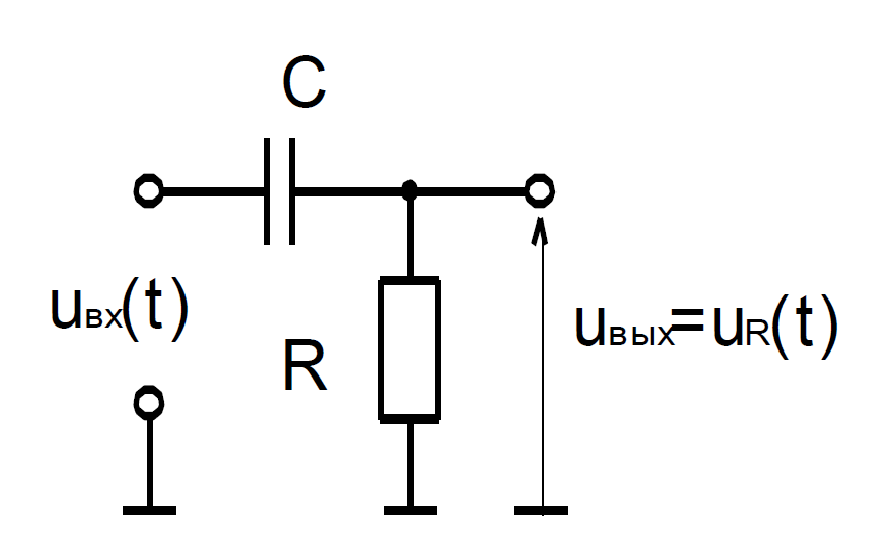
\includegraphics[scale=0.27]{diff.png}
\caption{Дифференцирующая\\ цепь}\label{figure:2.1:a}
\end{subfigure}
\begin{subfigure}[b]{0.35\textwidth}
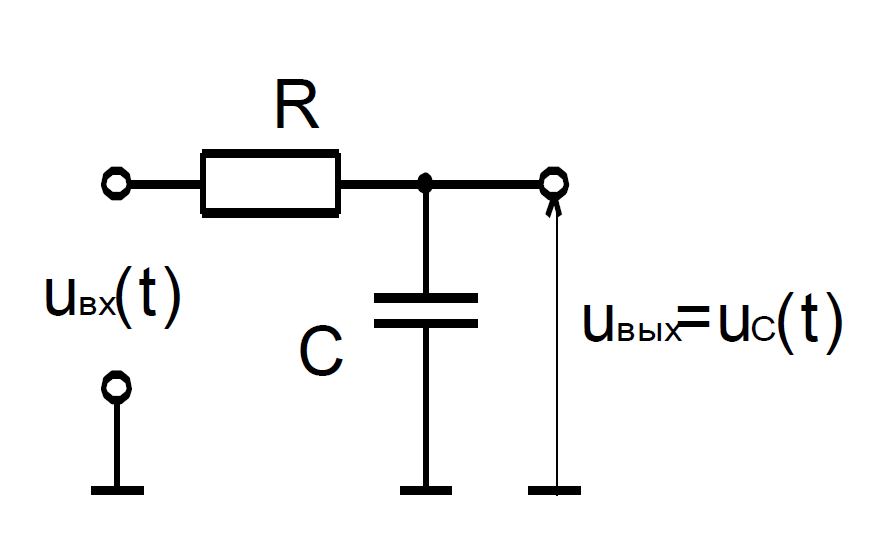
\includegraphics[scale=0.27]{int.png}
\caption{Интегрирующая\\ цепь}\label{figure:2.1:b}
\end{subfigure}
\end{figure}

На рисунке \ref{figure:2.1:a} изображена дифференцирующая RC-цепь, на \ref{figure:2.1:b} - интегрирующая RC-цепь.


\section{Исходные данные}

Выбранные исходные значения приведены в таблице \ref{tab:3:1}.

\begin{table}[H]
	\begin{center}
	\caption{Исходные данные}
	\def\arraystretch{1.2}
		\begin{tabular}{|c|c|c|c|c|c|c|}
			\hline 
			№ & Тип цепи & $U_\text{имп}$, B & R, кОм & С, нФ & $t_\text{имп}$, $\mu c$ & Q\\ 
			\hline 
			1 & Дифф & 10 & 10 & 0.1 & 10 & 10\\ 
			\hline 
			2 & Дифф & 10 & 10 & 1 & 10 & 10\\ 
			\hline 
			3 & Дифф & 10 & 10 & 10 & 10 & 10\\ 
			\hline 
			4 & Инт & 10 & 10 & 0.1 & 10 & 10\\ 
			\hline 
			5 & Инт & 10 & 10 & 1 & 10 & 10\\ 
			\hline 
			6 & Инт & 10 & 10 & 10 & 10 & 10\\
			\hline 
			7 & Инт & 10 & 10 & 10 & 10 & 5\\ 
			\hline 
			8 & Инт & 10 & 10 & 10 & 10 & 3\\ 
			\hline
		\end{tabular}
		\label{tab:3:1}
	\end{center}
\end{table}

\section{Теоретические зависимости}

Рассчитаем теоретические занчения $U_R(t)$ и $U_C(T)$ для дифференцирующей и интегрирующей RC-цепей.

\subsection{Расчетные формулы}

\begin{itemize}

\item Входное напряжение:
\begin{equation}
U_\text{вх} = \{(0 \text{ при } t < 0); (U_\text{имп} \text{ при } 0 \leq t \leq t_\text{имп}); (0 \text{ при } t \geq t_\text{имп})\}
\end{equation}

\item Выходное напряжение:

\begin{enumerate}
\item Для дифференцирующей цепи
\begin{equation}
U_R(t) = [U_C(\infty) - U_C(0)] \cdot e^{-\frac{t}{\tau}}
\end{equation}

\item Для интегрирующей цепи
\begin{equation}
U_C(t) = [U_C(0) - U_C(\infty)] \cdot e^{-\frac{t}{\tau}} + U_C(\infty)
\end{equation}

\end{enumerate}
\end{itemize}

\subsection{Расчеты для дифференцирующей RC-цепи}

\subsubsection{C = 0.1 нФ}

		$\tau = R \cdot C = 10 \cdot 10^3 \cdot 0.1 \cdot 10^{-9} = 10^{-6}$ (c)
		
		$t_\text{имп} = 10^{-5}$ (c)
		
\begin{itemize}
\item[] а) этап заряда конденсатора

		$U_C(0)	= 0,\ \ U_C(\infty) = U_\text{имп}$\\
		$U_R(t) = [U_\text{имп} - 0] \cdot e^{-\frac{t}{\tau}} = [10 - 0] \cdot e^{-\frac{t}{10^{-6}}} = 10 \cdot e^{-\frac{t}{10^{-6}}}$\\
		$U_R(0) = 10 \cdot e^{-\frac{0}{10^{-6}}} = 10 \cdot e^0 = 10$ (В)\\
		$U_R(t_\text{имп}) = 10 \cdot e^{-\frac{10^{-5}}{10^{-6}}} = 10 \cdot e^{-10} = 0$ (В)\\

\item[] б) этап разряда конденсатора
		
		$U_C(0)	= U_\text{имп},\ \ U_C(\infty) = 0$\\		
		$U_R(t) = [0 - U_\text{имп}] \cdot e^{-\frac{t}{\tau}} = [0 - 10] \cdot e^{-\frac{t}{10^{-6}}} = -10 \cdot e^{-\frac{t}{10^{-6}}}$\\
		$U_R(0) = -10 \cdot e^{-\frac{0}{10^{-6}}} = -10 \cdot e^0 = -10$\\
		Выберем такое $t$, что $t \gg \tau$, например, $t = 10 \cdot \tau$ \\
		$U_R(10 \cdot \tau) = -10 \cdot e^{-\frac{10^{-5}}{10^{-6}}} = -10 \cdot e^{-10} = 0$ (В)\\
		
\end{itemize}

\subsubsection{C = 1 нФ}

		$\tau = R \cdot C = 10 \cdot 10^3 \cdot 10^{-9} = 10^{-5}$ (c)
		
		$t_\text{имп} = 10^{-5}$ (c)

\begin{itemize}
\item[] а) этап заряда конденсатора

		$U_C(0)	= 0,\ \ U_C(\infty) = U_\text{имп}$\\
		$U_R(t) = [U_\text{имп} - 0] \cdot e^{-\frac{t}{\tau}} = [10 - 0] \cdot e^{-\frac{t}{10^{-5}}} = 10 \cdot e^{-\frac{t}{10^{-5}}}$\\
		$U_R(0) = 10 \cdot e^{-\frac{0}{10^{-5}}} = 10 \cdot e^0 = 10$ (В)\\
		$U_R(t_\text{имп}) = 10 \cdot e^{-\frac{10^{-5}}{10^{-5}}} = 10 \cdot e^{-1} = 3.679$ (В)\\

\item[] б) этап разряда конденсатора

		$U_C(0)	= U_\text{имп} - U_R(t),\ \ U_C(\infty) = 0$\\
		$U_R(t) = [0 - (U_\text{имп} - U_R(t))] \cdot e^{-\frac{t}{\tau}} = [0 - (10 - 3.679)] \cdot e^{-\frac{t}{10^{-5}}} = -6.32 \cdot e^{-\frac{t}{10^{-5}}}$\\
		$U_R(0) = -6.321 \cdot e^{-\frac{0}{10^{-5}}} = -6.321 \cdot e^0 = -6.321$ (В)\\
		Выберем такое $t$, что $t \gg \tau$, например, $t = 10 \cdot \tau$ \\
		$U_R(10 \cdot \tau)	= -6.321 \cdot e^{-\frac{10^{-4}}{10^{-5}}} = -6.321 \cdot e^{-10} = 0$ (В)\\
		
\end{itemize}

\subsubsection{C = 10 нФ}

		$\tau = R \cdot C = 10 \cdot 10^3 \cdot 10 \cdot 10^{-9} = 10^{-4}$ (c)
		
		$t_\text{имп} = 10^{-5}$ (c)

\begin{itemize}
\item[] а) этап заряда конденсатора

		$U_C(0)	= U_\text{имп},\ \ U_C(\infty) = 0$\\		
		$U_R(t) = [0 - U_\text{имп}] \cdot e^{-\frac{t}{\tau}} = [10 - 0] \cdot e^{-\frac{t}{10^{-4}}} = 10 \cdot e^{-\frac{t}{10^{-4}}}$\\
		$U_R(0) = 10 \cdot e^{-\frac{0}{10^{-4}}} = 10 \cdot e^0 = 10$ (В)\\
		$U_R(t_\text{имп}) = 10 \cdot e^{-\frac{10^{-5}}{10^{-4}}} = 10 \cdot e^{-0.1} = 9.048$ (В)\\

\item[] б) этап разряда конденсатора
		
		$U_C(0)	= U_\text{имп} - U_R(t),\ \ U_C(\infty) = 0$\\
		$U_R(t) = [0 - (U_\text{имп} - U_R(t))] \cdot e^{-\frac{t}{\tau}} = [0 - (10 - 9.048)] \cdot e^{-\frac{t}{10^{-4}}} = -0.952 \cdot e^{-\frac{t}{10^{-4}}}$\\
		$U_R(t) = -0.952 \cdot e^{-\frac{0}{10^{-4}}} = -0.952 \cdot e^0 = -0.952$ (В)\\
		Выберем такое $t$, что $t \gg \tau$, например, $t = 10 \cdot \tau$ \\
		$U_R(t) = -0.952 \cdot e^{-\frac{10^{-3}}{10^{-4}}} = -0.952 \cdot e^{-10} = 0$ (В)\\
		
\end{itemize}

\subsection{Расчеты для интегрирующей RC-цепи}

\subsubsection{C = 0.1 нФ, Q = 10}

		$\tau = R \cdot C = 10 \cdot 10^3 \cdot 0.1 \cdot 10^{-9} = 10^{-6}$ (c)
		
		$t_\text{имп} = 10^{-5}$ (c)
		
		$Q = 10$		
		
		$t_\text{п} = (Q - 1) \cdot t_\text{имп} = (10 - 1) \cdot 10^{-5} = 9 \cdot 10^{-5}$ (c)
		
\begin{itemize}
\item[] а) этап заряда конденсатора

		$U_C(0) = 0,\ \ U_C(\infty) = U_\text{имп}$\\
		$U_C(t) = [0 - U_\text{имп}] \cdot e^{-\frac{t}{\tau}} + U_\text{имп} = -10 \cdot e^{-\frac{t}{10^{-6}}} + 10$\\
		$U_C(0) = -10 \cdot e^{-\frac{0}{10^{-6}}} + 10 = -10 \cdot e^0 + 10 = 0$ (В)\\
		$U_C(t_\text{имп}) = -10 \cdot e^{-\frac{10^{-5}}{10^{-6}}} + 10 = -10 \cdot e^{-10} + 10 = 10$ (В)\\

\item[] б) этап разряда конденсатора
		
		$\frac{\tau}{t_\text{имп}} = \frac{10^{-6}}{10^{-5}} = 0.1 < 0.33 \Rightarrow U_C(0) = U_\text{имп},\ \ U_C(\infty) = 0$\\
		$U_C(t) = [U_\text{имп} - 0] \cdot e^{-\frac{t}{\tau}} + 0 = 10 \cdot e^{-\frac{t}{10^{-6}}}$\\
		$U_C(0) = 10 \cdot e^{-\frac{0}{10^{-6}}} = 10 \cdot e^0 = 10$ (В)\\
		$U_C(t_\text{п}) = 10 \cdot e^{-\frac{9 \cdot 10^{-5}}{10^{-6}}} = 10 \cdot e^{-90} = 0$ (В)\\
		
\end{itemize}

\subsubsection{C = 1 нФ, Q = 10}

		$\tau = R \cdot C = 10 \cdot 10^3 \cdot 10^{-9} = 10^{-5}$ (c)
		
		$t_\text{имп} = 10^{-5}$ (c)
		
		$Q = 10$		
		
		$t_\text{п} = (Q - 1) \cdot t_\text{имп} = (10 - 1) \cdot 10^{-5} = 9 \cdot 10^{-5}$ (c)

\begin{itemize}
\item[] а) этап заряда конденсатора

		$U_C(0) = 0,\ \ U_C(\infty) = U_\text{имп}$\\
		$U_C(t) = [0 - U_\text{имп}] \cdot e^{-\frac{t}{\tau}} + U_\text{имп} = -10 \cdot e^{-\frac{t}{10^{-5}}} + 10$\\
		$U_C(0) = -10 \cdot e^{-\frac{0}{10^{-5}}} + 10 = -10 \cdot e^0 + 10 = 0$ (В)\\
		$U_C(t_\text{имп}) = -10 \cdot e^{-\frac{10^{-5}}{10^{-5}}} + 10 = -10 \cdot e^{-1} + 10 = 6.321$ (В)\\

\item[] б) этап разряда конденсатора

		$\frac{\tau}{t_\text{имп}} = \frac{10^{-5}}{10^{-5}} = 1 > 0.33 \Rightarrow U_C(0) = U_C(t_\text{имп}),\ \ U_C(\infty) = 0$\\
		$U_C(t) = [U_C(t_\text{имп}) - 0] \cdot e^{-\frac{t}{\tau}} + 0 =  [6.321 - 0] \cdot e^{-\frac{t}{10^{-5}}} = 6.321 \cdot e^{-\frac{t}{10^{-5}}}$\\
		$U_C(0) = 6.321 \cdot e^{-\frac{0}{10^{-5}}} = 6.321 \cdot e^0 = 6.321$ (В)\\
		$U_C(t_\text{п}) = 6.321 \cdot e^{-\frac{9 \cdot 10^{-5}}{10^{-5}}} = 6.321 \cdot e^{-9} = 0$ (В)\\
		
\end{itemize}

\subsubsection{C = 10 нФ, Q = 10}

		$\tau = R \cdot C = 10 \cdot 10^3 \cdot 10 \cdot 10^{-9} = 10^{-4}$ (c)
		
		$t_\text{имп} = 10^{-5}$ (c)
		
		$Q = 10$		
		
		$t_\text{п} = (Q - 1) \cdot t_\text{имп} = (10 - 1) \cdot 10^{-5} = 9 \cdot 10^{-5}$ (c)

\begin{itemize}
\item[] а) этап заряда конденсатора

		$U_C(0) = 0,\ \ U_C(\infty) = U_\text{имп}$\\	
		$U_C(t) = [0 - U_\text{имп}] \cdot e^{-\frac{t}{\tau}} + U_\text{имп} = [0 - 10] \cdot e^{-\frac{t}{10^{-4}}} + 10 = -10 \cdot e^{-\frac{t}{10^{-4}}} + 10$\\
		$U_C(0) = -10 \cdot e^{-\frac{0}{10^{-4}}} + 10 = 0$ (В)\\
		$U_C(t_\text{имп}) = -10 \cdot e^{-\frac{10^{-5}}{10^{-4}}} + 10 = -10 \cdot e^{-0.1} + 10 = 0.952$ (В)\\
		
\item[] б) этап разряда конденсатора
	
		$\frac{\tau}{t_\text{имп}} = \frac{10^{-4}}{10^{-5}} = 10 > 0.33 \Rightarrow U_C(0) = U_C(t_\text{имп}),\ \ U_C(\infty) = 0$\\
		$U_C(t) = [U_C(t_\text{имп}) - 0] \cdot e^{-\frac{t}{\tau}} + 0 =  [0.952 - 0] \cdot e^{-\frac{t}{10^{-4}}} = 0.952 \cdot e^{-\frac{t}{10^{-4}}}$\\
		$U_C(0) = 0.952 \cdot e^{-\frac{0}{10^{-4}}} = 0.952 \cdot e^0 = 0.952$ (В)\\
		$U_C(t_\text{п}) = 0.952 \cdot e^{-\frac{9 \cdot 10^{-5}}{10^{-4}}} = 0.952 \cdot e^{-0.9} = 0.387$ (В)\\
		
\end{itemize}

	За время паузы между импульсами конденсатор не успевает полностью разрядиться. Повторим расчеты, пока не не наступит установившийся процесс, т.е. результаты расчета на предыдущем и последующем этапе будут совпадать. Воспользуемся итерационной формулой.
\begin{table}[H]

	\begin{center}
	\caption{Значения напряжения при времени, равном $0$ и $t_\text{имп}$, полученные по итерационной формуле}
	\def\arraystretch{1.2}
	\begin{tabular}{|c|c||c|c|}
		\hline 
		$U_C(0)$, В & $U_C(t_\text{имп})$, В & $U_C(0)$, В & $U_C(t_\text{имп})$, \\ 
		\hline 
		0.387 & 0.952 & 0.610 & 1.502 \\
		\hline 
		0.529 & 1.302 & 0.612 & 1.504 \\
		\hline 
		0.582 & 1.430 & 0.612 & 1.505 \\ 
		\hline 
		0.601 & 1.478 & 0.612 & 1.505 \\
		\hline 
		0.608 & 1.495 & & \\
		\hline 
		\end{tabular} 	
		
	\end{center}
\end{table}
	Результаты двух последних вычислений совпадают, следовательно процесс установился. Получаем:
	
	$U_C(0) = 0.612$ (В)
	
	$U_C(t_\text{имп}) = 1.505$ (В)
	
\subsubsection{C = 10 нФ, Q = 5}

		$\tau = R \cdot C = 10 \cdot 10^3 \cdot 10 \cdot 10^{-9} = 10^{-4}$ (c)
		
		$t_\text{имп} = 10^{-5}$ (c)
		
		$Q = 5$		
		
		$t_\text{п} = (Q - 1) \cdot t_\text{имп} = (5 - 1) \cdot 10^{-5} = 4 \cdot 10^{-5}$ (c)
		
		
\begin{itemize}
\item[] а) этап заряда конденсатора

		$U_C(0) = 0,\ \ U_C(\infty) = U_\text{имп}$\\	
		$U_C(t) = [0 - U_\text{имп}] \cdot e^{-\frac{t}{\tau}} + U_\text{имп} = [0 - 10] \cdot e^{-\frac{t}{10^{-4}}} + 10 = -10 \cdot e^{-\frac{t}{10^{-4}}} + 10$\\
		$U_C(0) = -10 \cdot e^{-\frac{0}{10^{-4}}} + 10 = 0$ (В)\\
		$U_C(t_\text{имп}) = -10 \cdot e^{-\frac{10^{-5}}{10^{-4}}} + 10 = -10 \cdot e^{-0.1} + 10 = 0.952$ (В)\\
		
\item[] б) этап разряда конденсатора
	
		$\frac{\tau}{t_\text{имп}} = \frac{10^{-4}}{10^{-5}} = 10 > 0.33 \Rightarrow U_C(0) = U_C(t_\text{имп}),\ \ U_C(\infty) = 0$\\
		$U_C(t) = [U_C(t_\text{имп}) - 0] \cdot e^{-\frac{t}{\tau}} + 0 =  [0.952 - 0] \cdot e^{-\frac{t}{10^{-4}}} = 0.952 \cdot e^{-\frac{t}{10^{-4}}}$\\
		$U_C(0) = 0.952 \cdot e^{-\frac{0}{10^{-4}}} = 0.952 \cdot e^0 = 0.952$ (В)\\
		$U_C(t_\text{п}) = 0.952 \cdot e^{-\frac{4 \cdot 10^{-5}}{10^{-4}}} = 0.952 \cdot e^{-0.4} = 0.638$ (В)\\
		
\end{itemize}				
		
За время паузы между импульсами конденсатор не успевает полностью разрядиться. Повторим расчеты, пока не не наступит установившийся процесс, т.е. результаты расчета на предыдущем и последующем этапе будут совпадать.	Воспользуемся итерационной формулой.
\begin{table}[H]

	\begin{center}
	\caption{Значения напряжения при времени, равном $0$ и $t_\text{имп}$, полученные по итерационной формуле}
	\def\arraystretch{1.2}
	\begin{tabular}{|c|c||c|c|}
		\hline 
		$U_C(0)$, В & $U_C(t_\text{имп})$, В & $U_C(0)$, В & $U_C(t_\text{имп})$, В \\ 
		\hline 
		0.638 & 0.952 & 1.610 & 2.402 \\ 
		\hline 
		1.025 & 1.529 & 1.614 & 2.409 \\ 
		\hline 
		1.259 & 1.879 & 1.617 & 2.412 \\ 
		\hline 
		1.402 & 2.091 & 1.619 & 2.415 \\ 
		\hline 
		1.488 & 2.220 & 1.620 & 2.416 \\
		\hline 
		1.540 & 2.298 & 1.620 & 2.417 \\ 
		\hline 
		1.572 & 2.346 & 1.621 & 2.418 \\ 
		\hline 
		1.592 & 2.374 & 1.621 & 2.418 \\ 
		\hline 
		1.603 & 2.392 & & \\
		\hline
		\end{tabular} 	
		
	\end{center}
\end{table}
	Результаты двух последних вычислений совпадают, следовательно процесс установился. Получаем:
	
	$U_C(0) = 1.621$ (В)	
	
	$U_C(t_\text{имп}) = 2.418$ (В)
	

\subsubsection{C = 10 нФ, Q = 3}

$\tau = R \cdot C = 10 \cdot 10^3 \cdot 10 \cdot 10^{-9} = 10^{-4}$ (c)
		
		$t_\text{имп} = 10^{-5}$ (c)
		
		$Q = 3$
		
		$t_\text{п} = (Q - 1) \cdot t_\text{имп} = (3 - 1) \cdot 10^{-5} = 2 \cdot 10^{-5}$ (c)
		
		
\begin{itemize}
\item[] а) этап заряда конденсатора

		$U_C(0) = 0,\ \ U_C(\infty) = U_\text{имп}$\\	
		$U_C(t) = [0 - U_\text{имп}] \cdot e^{-\frac{t}{\tau}} + U_\text{имп} = [0 - 10] \cdot e^{-\frac{t}{10^{-4}}} + 10 = -10 \cdot e^{-\frac{t}{10^{-4}}} + 10$\\
		$U_C(0) = -10 \cdot e^{-\frac{0}{10^{-4}}} + 10 = 0$ (В)\\
		$U_C(t_\text{имп}) = -10 \cdot e^{-\frac{10^{-5}}{10^{-4}}} + 10 = -10 \cdot e^{-0.1} + 10 = 0.952$ (В)\\
		
\item[] б) этап разряда конденсатора
	
		$\frac{\tau}{t_\text{имп}} = \frac{10^{-4}}{10^{-5}} = 10 > 0.33 \Rightarrow U_C(0) = U_C(t_\text{имп}),\ \ U_C(\infty) = 0$\\
		$U_C(t) = [U_C(t_\text{имп}) - 0] \cdot e^{-\frac{t}{\tau}} + 0 =  [0.952 - 0] \cdot e^{-\frac{t}{10^{-4}}} = 0.952 \cdot e^{-\frac{t}{10^{-4}}}$\\
		$U_C(0) = 0.952 \cdot e^{-\frac{0}{10^{-4}}} = 0.952 \cdot e^0 = 0.952$ (В)\\
		$U_C(t_\text{п}) = 0.952 \cdot e^{-\frac{ 2 \cdot 10^{-5}}{10^{-4}}} = 0.952 \cdot e^{-0.2} = 0.779$ (В)\\
		
\end{itemize}				
		
За время паузы между импульсами конденсатор не успевает полностью разрядиться. Повторим расчеты, пока не не наступит установившийся процесс, т.е. результаты расчета на предыдущем и последующем этапе будут совпадать.	Воспользуемся итерационной формулой.
\begin{table}[H]

	\begin{center}
	\caption{Значения напряжения при времени, равном $0$ и $t_\text{имп}$, полученные по итерационной формуле}
	\begin{tabular}{|c|c||c|c|}
		\hline 
		$U_C(0)$, В & $U_C(t_\text{имп})$, В & $U_C(0)$, В & $U_C(t_\text{имп})$, В\\ 
		\hline 
		0.779 & 0.952 & 2.981 & 3.641 \\ 
		\hline 
		1.356 & 1.657 & 2.988 & 3.649 \\ 
		\hline 
		1.784 & 2.179 & 2.992 & 3.655 \\
		\hline 
		2.101 & 2.566 & 2.996 & 3.659 \\
		\hline 
		2.335 & 2.852 & 2.999 & 3.662 \\ 
		\hline 
		2.509 & 3.065 & 3.000 & 3.665 \\
		\hline 
		2.638 & 3.222 & 3.002 & 3.667 \\
		\hline 
		2.733 & 3.338 & 3.003 & 3.668 \\ 
		\hline 
		2.804 & 3.425 & 3.004 & 3.669 \\
		\hline 
		2.856 & 3.489 & 3.004 & 3.670 \\
		\hline 
		2.895 & 3.536 & 3.005 & 3.670 \\ 
		\hline 
		2.924 & 3.571 & 3.005 & 3.670 \\ 
		\hline 
		2.945 & 3.597 & 3.005 & 3.671 \\ 
		\hline 
		2.961 & 3.612 & 3.006 & 3.671 \\ 
		\hline 
		2.973 & 3.631 & 3.006 & 3.671 \\ 
		\hline 
		\end{tabular}  	
		
	\end{center}
\end{table}
	Результаты двух последних вычислений совпадают, следовательно процесс установился. Получаем:
	
	$U_C(0) = 3.006$ (В)
	
	$U_C(t_\text{имп}) = 3.671$ (В)

\section{Экспериментально снятые зависимости}

\begin{figure}[H]
	\begin{center}
		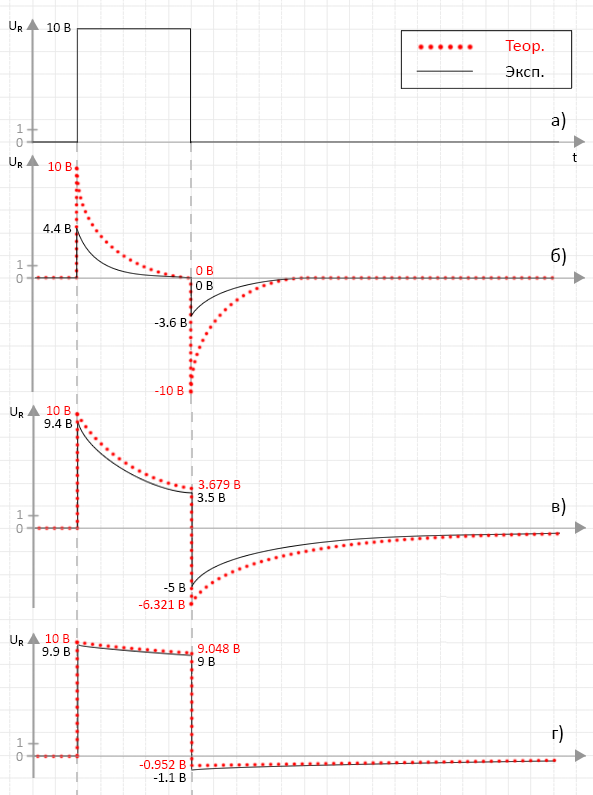
\includegraphics[width=14cm]{img/diff_with_theory2}
		\caption{Эксперементальная диаграмма входного и выходного импульса для дифференцирующей цепи при $R = 10$ кОм и: б) $C = 0.1$ нФ; в) $C = 1$ нФ; г) $C = 10$ нФ.} 
		\label{d:1} % название для ссылок внутри кода
	\end{center}
\end{figure}

\begin{figure}[H]
	\begin{center}
		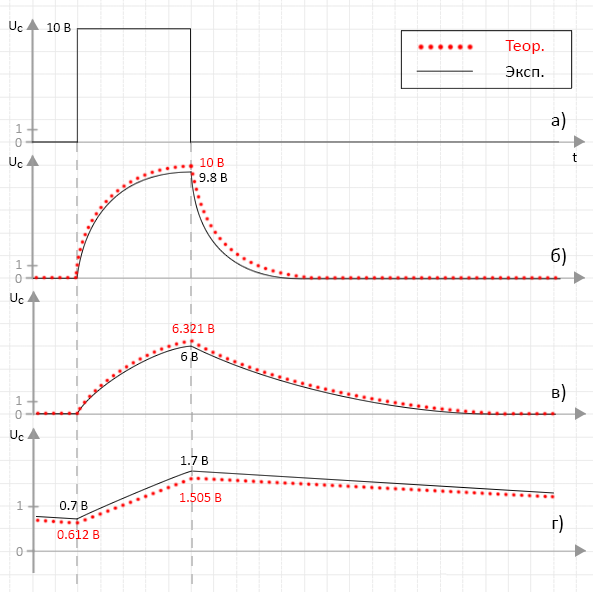
\includegraphics[width=14cm]{img/int_with_theory}
		\caption{Эксперементальная диаграмма входного и выходного импульса для интегрирующей цепи при $R = 1$ кОм и: б) $C = 0.1$ нФ; в) $C = 1$ нФ; г) $C = 10$ нФ.} 
		\label{i:1} % название для ссылок внутри кода
	\end{center}
\end{figure}

\begin{figure}[H]
	\begin{center}
		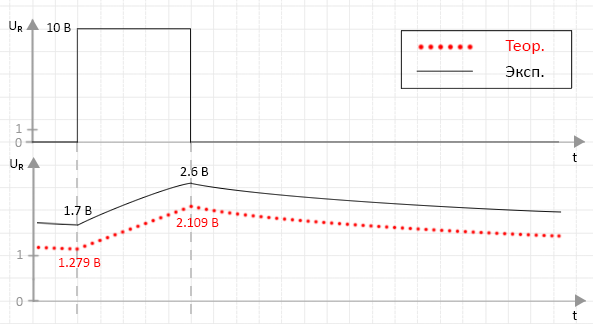
\includegraphics[width=14cm]{img/q5_with_theory}
		\caption{Эксперементальная диаграмма входного и выходного импульса для интегрирующей цепи при $R = 1$ кОм, $C = 10$ нФ и $Q = 5$.} 
		\label{i:2} % название для ссылок внутри кода
	\end{center}
\end{figure}

\begin{figure}[H]
	\begin{center}
		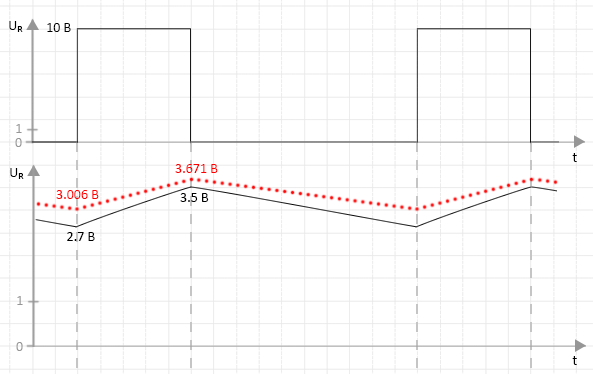
\includegraphics[width=14cm]{img/q3_with_theory}
		\caption{Эксперементальная диаграмма входного и выходного импульса для интегрирующей цепи при $R = 1$ кОм, $C = 10$ нФ и $Q = 3$.}
		\label{i:3} % название для ссылок внутри кода
	\end{center}
\end{figure}

\section{Погрешности}

\subsection{Предельно допустимые погрешности}

\begin{center}
$\delta R = 0.1 = 10\%$\\
$\delta C = 0.1 = 10\%$\\
\end{center}

Дифференцирующая и интегрирующая цепи включают в себя по одному резистору и по одному конденсатору, поэтому предельно допустимая погрешность $U_0$ вычисляется следующим образом:


$\delta U_0 = \sqrt{(\delta R)^2 + (\delta C)^2} = \sqrt{0.1^2 + 0.1^2} = \sqrt{0.02} = 0.141 = 14.1 \%$

\subsection{Погрешности результатов эксперемента} %заменить epsilon на delta

Отклонение эксперементально полученных данных от теоретических рассчитывается по формуле:

\begin{equation}
		\delta U = \Bigl |\frac{U\text{теор}-U\text{эксп}}{U\text{теор}}\Bigl |
\end{equation}

\subsection{Дифференцирующая цепь}
\subsubsection{C = 0.1 нФ, Q = 10}
\begin{itemize}
\item[] а) $t = 0$
	
		$\delta U = \Bigl | \frac{U_{R_\text{теор}}(0) - U_{R_\text{эксп}}(0)}{U_{R_\text{теор}}(0)} \Bigl | = \Bigl | \frac{10 - 4.4}{10} \Bigl | = 0.56 = 56\% > \delta U_0 = 14.1\%$

\item[] б) $t = t_\text{имп}-0$

		$\delta U = \Bigl | \frac{U_{R_\text{теор}}(t_\text{имп}-0) - U_{R_\text{эксп}}(t_\text{имп}-0)}{U_{R_\text{теор}}(t_\text{имп}-0)} \Bigl | = \Bigl | \frac{0 - 0}{0} \Bigl | = 0 = 0\% < \delta U_0 = 14.1\%$

\item[] в)  $t = t_\text{имп}+0$

		$\delta U = \Bigl | \frac{U_{R_\text{теор}}(t_\text{имп}+0) - U_{R_\text{эксп}}(t_\text{имп}+0)}{U_{R_\text{теор}}(t_\text{имп}+0)} \Bigl | = \Bigl | \frac{-10 - (-4.4)}{-10} \Bigl | = 0.64 = 64\% > \delta U_0 = 14.1\%$

\end{itemize}

\subsubsection{C = 1 нФ, Q = 10}
\begin{itemize}
\item[] а)  $t = 0$

		$\delta U = \Bigl | \frac{U_{R_\text{теор}}(0) - U_{R_\text{эксп}}(0)}{U_{R_\text{теор}}(0)} \Bigl | = \Bigl | \frac{10 - 9.4}{10} \Bigl | = 0.06 = 6\% < \delta U_0 = 14.1\%$

\item[] б) $t = t_\text{имп}-0$

		$\delta U = \Bigl | \frac{U_{R_\text{теор}}(t_\text{имп}-0) - U_{R_\text{эксп}(t_\text{имп}}-0)}{U_{R_\text{теор}}(t_\text{имп}-0)} \Bigl | = \Bigl | \frac{3.679 - 3.5}{3.679} \Bigl | = 0.049 = 4.9\% < \delta U_0 = 14.1\%$

\item[] в) $t = t_\text{имп}+0$

		$\delta U = \Bigl | \frac{U_{R_\text{теор}}(t_\text{имп}+0) - U_{R_\text{эксп}}(t_\text{имп}+0)}{U_{R_\text{теор}}(t_\text{имп}+0)} \Bigl | = \Bigl | \frac{-6.321 - (-5)}{-6.321} \Bigl | = 0.209 = 20.9\% > \delta U_0 = 14.1\%$

\end{itemize}

\subsubsection{C = 10 нФ, Q = 10}
\begin{itemize}
\item[] а) $t = 0$

		$\delta U = \Bigl | \frac{U_{R_\text{теор}}(0) - U_{R_\text{эксп}}(0)}{U_{R_\text{теор}(0)}} \Bigl | = \Bigl | \frac{10 - 9.9}{10} \Bigl | = 0.01 = 1\% < \delta U_0 = 14.1\%$

\item[] б) $t = t_\text{имп}-0$

		$\delta U = \Bigl | \frac{U_{R_\text{теор}}(t_\text{имп}-0) - U_{R_\text{эксп}}(t_\text{имп}-0)}{U_{R_\text{теор}}(t_\text{имп}-0)} \Bigl | = \Bigl | \frac{9.048 - 9}{9.048} \Bigl | = 0.005 = 0.5\% < \delta U_0 = 14.1\%$

\item[] в) $t = t_\text{имп}+0$

		$\delta U = \Bigl | \frac{U_{R_\text{теор}}(t_\text{имп}+0) - U_{R_\text{эксп}}(t_\text{имп}+0)}{U_{R_\text{теор}}(t_\text{имп}+0)} \Bigl | = \Bigl | \frac{-0.952 - (-1.1)}{-0.952} \Bigl | = 0.155 = 15.5\% \simeq \delta U_0 = 14.1\%$

\end{itemize}

\subsection{Интегрируюшая цепь}
\subsubsection{C = 0.1 нФ, Q = 10}
\begin{itemize}

\item[] а) $t = 0$

		$\delta U = \Bigl | \frac{U_{C_\text{теор}}(0) - U_{C_\text{эксп}}(0)}{U_{C_\text{теор}(0)}} \Bigl | = \Bigl | \frac{0 - 0}{0} \Bigl | = 0 = 0\% < \delta U_0 = 14.1\%$

\item[] б) $t = t_\text{имп}$

		$\delta U = \Bigl | \frac{U_{C_\text{теор}}(t_\text{имп}) - U_{C_\text{эксп}}(t_\text{имп})}{U_{C_\text{теор}}(t_\text{имп})} \Bigl | = \Bigl | \frac{10 - 9.8}{10} \Bigl | = 0.02 = 2\% < \delta U_0 = 14.1\%$

\end{itemize}

\subsubsection{C = 1 нФ, Q = 10}
\begin{itemize}

\item[] а) $t = 0$

		$\delta U = \Bigl | \frac{U_{C_\text{теор}}(0) - U_{C_\text{эксп}}(0)}{U_{C_\text{теор}(0)}} \Bigl | = \Bigl | \frac{0 - 0}{0} \Bigl | = 0 = 0\% < \delta U_0 = 14.1\%$

\item[] б) $t = t_\text{имп}$

		$\delta U = \Bigl | \frac{U_{C_\text{теор}}(t_\text{имп}) - U_{C_\text{эксп}}(t_\text{имп})}{U_{C_\text{теор}}(t_\text{имп})} \Bigl | = \Bigl | \frac{6.321 - 6}{6.321} \Bigl | = 0.051 = 5.1\% < \delta U_0 = 14.1\%$

\end{itemize}

\subsubsection{C = 10 нФ, Q = 10}
\begin{itemize}

\item[] а) $t = 0$

		$\delta U = \Bigl | \frac{U_{C_\text{теор}}(0) - U_{C_\text{эксп}}(0)}{U_{C_\text{теор}(0)}} \Bigl | = \Bigl | \frac{0.612 - 0.7}{0.612} \Bigl | = 0.144 = 14.4\% \simeq \delta U_0 = 14.1\%$

\item[] б) $t = t_\text{имп}$

		$\delta U = \Bigl | \frac{U_{C_\text{теор}}(t_\text{имп}) - U_{C_\text{эксп}}(t_\text{имп})}{U_{C_\text{теор}}(t_\text{имп})} \Bigl | = \Bigl | \frac{1.505 - 1.7}{1.505} \Bigl | = 0.13 = 13\% < \delta U_0 = 14.1\%$

\end{itemize}

\subsubsection{C = 10 нФ, Q = 5}
\begin{itemize}

\item[] а) $t = 0$

		$\delta U = \Bigl | \frac{U_{C_\text{теор}}(0) - U_{C_\text{эксп}}(0)}{U_{C_\text{теор}(0)}} \Bigl | = \Bigl | \frac{1.621 - 1.7}{1.621} \Bigl | = 0.049 = 4.9\% < \delta U_0 = 14.1\%$

\item[] б) $t = t_\text{имп}$

		$\delta U = \Bigl | \frac{U_{C_\text{теор}}(t_\text{имп}) - U_{C_\text{эксп}}(t_\text{имп})}{U_{C_\text{теор}}(t_\text{имп})} \Bigl | = \Bigl | \frac{2.418 - 2.6}{2.418} \Bigl | = 0.075 = 7.5\% < \delta U_0 = 14.1\%$

\end{itemize}

\subsubsection{C = 10 нФ, Q = 3}
\paragraph{C = 10 нФ, Q = 3}
\begin{itemize}

\item[] а) $t = 0$

		$\delta U = \Bigl | \frac{U_{C_\text{теор}}(0) - U_{C_\text{эксп}}(0)}{U_{C_\text{теор}(0)}} \Bigl | = \Bigl | \frac{3.006 - 2.7}{3.006} \Bigl | = 0.102 = 10.2\% < \delta U_0 = 14.1\%$

\item[] б) $t = t_\text{имп}$

		$\delta U = \Bigl | \frac{U_{C_\text{теор}}(t_\text{имп}) - U_{C_\text{эксп}}(t_\text{имп})}{U_{C_\text{теор}}(t_\text{имп})} \Bigl | = \Bigl | \frac{3.671 - 3.5}{3.671} \Bigl | = 0.046 = 4.6\% < \delta U_0 = 14.1\%$

\end{itemize}
  
\section{Выводы}

В результате эксперимента были получены на дифференцирующей RC-цепи значения: $U_{R}(0)$ при $C = 0.1$ нФ и $Q = 10$, приведенная погрешность которого 56\%; $U_{R}(t_\text{имп}+0)$ при $C = 0.1$ нФ и $Q = 10$, приведенная погрешность которого 64\%; $U_{R}(t_\text{имп}+0)$ при $C = 1$ нФ и $Q = 10$, приведенная погрешность которого 20.9\%; $U_{R}(t_\text{имп}+0)$ при $C = 10$ нФ и $Q = 10$, приведенная погрешность которого 15.5\%; и на интегрирующей RC-цепи значение $U_{C}(0)$ при $C = 10$ нФ и $Q = 10$, приведенная погрешность которого 14.4\%. Значения приведенных погрешностей в вышеуказанных случаях превышают значение предельно допустимой погрешности, которое равно 14.1\%. Это может быть объяснено тем, что теоретические формулы не учитывают, что осциллограф имеет входные сопротивление и электроемкость. 

В остальных случаях приведенные погрешности снятых во время эксперимента величин не превосходят предельно допустимую погрешность.

Итак, без учета влияния осциллографа на результаты измерений, метод исследования, используемый в данной лабораторной работе не является достаточно точным.

\end{document}
